\documentclass[a4paper]{article}
    \usepackage{geometry}
    \usepackage{amsmath,bm}
    \usepackage{indentfirst} %————首行缩进
    \setlength{\parindent}{2.0em} %————首行缩进
    \usepackage{setspace} %————调整行距
    \geometry{left=2.0cm,right=2.0cm,top=2.5cm,bottom=2.5cm}
    \usepackage{CJK}
    \usepackage{booktabs}
    \usepackage{graphicx}%————插图
    \usepackage{amsfonts} %————双线R
	\usepackage{mathrsfs} %————花体
    \renewcommand{\baselinestretch}{1.0}%————调整行距
    \begin{CJK}{UTF8}{gbsn}
    \renewcommand\tablename{表}
    \renewcommand\figurename{图}
       \title{计算机视觉中的深度学习文献综述}  %———总标题
\begin{document}
\maketitle % —— 显示标题
\author{Athanasios Voulodimos$^{1,2}$,}
\author{Nikolaos Doulamis$^{2}$,}
\author{Anastasios Doulamis$^{2}$,}
\author{Eftychios Protopapadakis$^{2}$}\\\\
$^{1}$雅典科技教育学院信息学系,12210,希腊,雅典\\
$^{2}$雅典国家技术大学,15780,希腊,雅典\\\\
信件写明收件人为Athanasios Voulodimos;thanosv@mail.ntua.gr\\\\
收稿日期:2017年6月17日;通过日期2017年11月27日;发表日期2018年2月1日\\\\
学术编辑:Diego Andina\\\\
版权所有\copyright2018 Athanasios Voulodimos等人。本文是在知识共享归属许可下开放共享的。知识共享归属许可协议允许其他人在合理引用原作的前提下,对原作无限制地使用、传播或复制。\\\\

\begin{abstract}
	近年来深度学习方法在各个领域中不断超越之前先进的机器学习技术,计算机视觉也是这些领域之一。本文概述了一些计算机视觉问题上最值得注意的深度学习方案,即卷积神经网络、深度波尔茨曼机、深度信念网络和多层降噪自动编码机,简述了它们的历史、结构、优点和局限性,并展现了它们在各种计算机视觉任务中的应用,例如目标检测、人脸识别、行为识别以及人体姿态估计,最后简要地总结了深度学习在计算机视觉领域未来的发展方向以及面临的挑战。
\end{abstract}
%\tableofcontents %—— 制作目录(目录是根据标题自动生成的)
\section{简介} %——一号子标题  China is in East Asia.
深度学习模型通过多个处理层对的信息进行多层抽象,从而模拟大脑提取出大型数据中错综复杂的信息。深度学习包含很多种研究方法,包括神经网络、多层概率模型以及各种各样的监督的和非监督的特征学习算法。近期的深度学习狂潮主要有两个原因,一是深度学习方法在各种任务中的表现都好过曾经的先进技术,二是各行各业产生了大量错综复杂的数据(如视觉数据,音频数据,医药数据,社会数据和传感器数据),为深度学习模型提供了大量训练数据。


为了创造一个可以模拟人脑的系统,人们点燃了神经网络发展的星星之火。1943年,McCulloch和Pitts$^{[1]}$尝试研究人脑通过简单的神经元来处理复杂任务的机制,他们创造的“The McCulloch and Pitts model of a neuron”(MCP模型)对人工神经网络的发展作出了重要贡献。神经网络领域中的主要贡献列举在表1中,其中包括了LeNet$^{[2]}$和长短时记忆网络$^{[3]}$等引领了当今的深度学习狂潮的神经网络。深度学习领域中最重大的突破之一是2006年Hinton等人$^{[4]}$提出的深度信念网络,这是一个多层的限制玻尔兹曼机,在非监督的模式下基于贪心法逐层训练。通过非监督模式引导中间层的学习,每层单独地训练是过去十几年来各种深度结构和深度学习算法背后的主要原理。

大规模、高质量、公开的带标签的数据集以及GPU的并行计算能力是促成深度学习繁荣的主要原因,其中使用GPU进行并行计算使运行在CPU的上模型可以转移到GPU上,从而大大加快了深度学习模型的训练速度。此外还有一些其他原因,比如不再使用饱和的激活函数(例如正弦函数,sigmoid函数)从而缓解梯度消失的问题,再如新的正则化方法的提出(例如dropout,batch normalization和数据增强),以及功能强大的深度学习框架TensorFlow$^{[7]}$,Theano和mxnet的出现,使得模型能更快地得到实现。
\linespread{1.5}
\begin{table}
	\caption{神经网络发展过程中的重要里程碑}
	\begin{tabular}{cc}
		\toprule  %添加表格头部粗线
		里程碑/贡献                            & 贡献者,时间                                       \\
		\midrule  %添加表格中横线
		MCP模型,被认为是人工神经网络的原型    & McCulloch \& Pitts,1943                           \\
		赫布学习法则                           & Hebb,1949                                         \\
		第一个感知器                           & Rosenblatt,1958                                   \\
		反向传播算法                           & Werbos,1974                                       \\
		新认知机,被认为是卷积神经网络的原型   & Fukushima,1980                                    \\
		玻尔兹曼机                             & Ackley,Hinton \& Sejnowski,1985                  \\
		限制玻尔兹曼机                         & Smolensky,1986                                    \\
		循环神经网络                           & Jordan,1986                                       \\
		自编码器                               & Rumelhart,Hinton \& Williams,1986,Ballard,1987 \\
		LeNet,开启了卷积神经网络的纪元        & LeCun,1990                                        \\
		长短记忆网络                           & Hochreiter \& Schmidhuber,1997                    \\
		深度信念网络,引领了深度学习的时代     & Hinton,2006                                       \\
		深度波尔茨曼机                         & Salakhutdinov \& Hinton,2009                      \\
		AlexNet,开创了CNN应用于图像分类的时代 & Krizhevsky,Sutskever,\& Hinton,2012             \\
		\bottomrule %添加表格底部粗线
	\end{tabular}
\end{table}

深度学习加快了计算机视觉领域各种问题的进展,比如目标检测[8,9],运动跟踪[10,11],行为识别[12,13],人体姿态估计[14,15]和语义分割[16,17]。本文会简明地概述计算机视觉应用中的深度学习结构和算法的发展。我们将重点讨论三种最重要的深度学习模型及其在计算机视觉中的应用,即卷积神经网络(CNNs),包括深度信念网络(DBNs)和深度玻尔兹曼机(DBMs)的“玻尔兹曼家族”和多层(降噪)自动编码机。显然,这些并不全面。比如,长短时记忆网络(LSTM),一种循环神经网络,在深度学习领域也有非凡的意义,但本文并不会讨论,因为LSTM主要应用于语言建模,文本分类,手写识别,机器翻译,语音/音乐分析,而更少地应用在计算机视觉领域。本文是为给计算机视觉和多媒体分析以及普通对计算机视觉任务使用的先进的深度学习方法感兴趣的研究者提供便利。

本文的剩余部分将按照如下安排。第二部分中,概述上文所述的三种深度学习模型:卷积神经网络,深度信念网络和深度玻尔兹曼机,以及多层自动编码机。本文将列举每种模型的基础结构、训练过程、近期发展、优点和缺点。第三部分中,本文会描述深度学习算法对关键的计算机视觉任务的贡献,比如目标检测和识别、人脸识别、行为识别和人体姿态估计。本文也会提供一个重要数据集和其来源的列表,以备评估和验证这些深度学习算法。最后,第四部分概述并总结这些研究成果。
\section{深度学习方法及其发展}
\subsection{卷积神经网络} %——二号子标题  Beijing is the capital of China.
卷积神经网络(CNNs)受到视觉系统结构的启发,特别地受到文献[18]中模型的启发。第一个基于局部连接神经元和图像的分层变换计算模型由Neocognitron[19]提出,这个模型说明了当权值相同的神经元作用在前一层不同位置神经元的输出时,模型可以习得一种平移不变量。Yann LeCun和他的合作者之后采用误差梯度设计出了卷积神经网络,并且在各种模式识别任务中取得了很好的结果[20-22]。

一个CNN主要包括三个神经层种类,即,(1)卷积层,(2)池化层,(3)全连接层。每种层在网络中起到不同的作用。图1展现了在目标检测任务中的一个CNN的结构。CNN的每层将输入经过神经元激活转化成输出,最终将输入引导到全连接层,结果把输入数据转化为一维的特征向量。CNNs在计算机视觉应用领域已经取得了巨大的成功,比如人脸检测,目标识别,机器人视觉和自动驾驶。\\
\begin{figure}[ht]
	\centering
	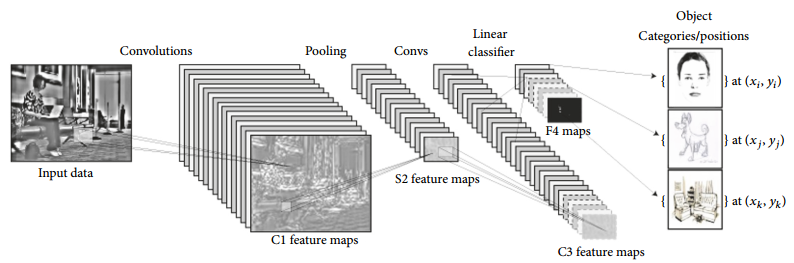
\includegraphics[scale=0.6]{fig1.png}
	\caption{CNN在计算机视觉任务(目标检测)中的一种结构}
	\label{fig:label}
\end{figure}
(1)卷积层\\
在卷积层中,CNN使用各种核对整个图像和每个特征图进行卷积,生成多个特征图。由于卷积运算的优势,很多研究结果[23,24]提出以它代替全连接层可以得到更快的训练速度。\\
(2)池化层\\
池化层是负责降低输入图像的维度(长×宽),以便输入到卷积层中,池化层不会影响输入的纵深维度。这一层的运算也被称作为二次抽样或下抽样。即便降维同时会导致信息的丢失,这种信息丢失对神经网络是有利的,因为输入规模的减小可以为之后的网络层减少计算开销,而且这样也可以防止过拟合。平均池化(average pooling)和最大池化(max pooling)是最常用的策略。在[25]中,对最大池化和平均池化的表现进行了细致的理论分析,而在[26]中,最大池化被验证会导致模型更快收敛,能够找到较好的不变特征,并提升模型的泛化性能。此外,当前的文献中有很多不同的池化层,每种都受到不同动机的启发并满足各种各样的需求,比如,随机池化(stochastic pooling)[27],空间金字塔赤化(spatial pyramid pooling)[28,29],以及def-pooling[30]。\\
(3)全连接层\\
在之前的卷积层和池化层之后,高级的推理能力将由全连接层实现。像它的名字一样,全连接层中的神经元与前一层的输出完全连接,因此它们的激活结果可以通过矩阵乘法和偏置偏移来计算。全连接层最终将二维的特征图转化为一维的特征向量。导出的向量可能被前向传播到一些分类器用以分类[31]或者被当做图片的特征向量用以后续处理[32]。

CNNs的结构采用了三个具体的思想:(a)局部感受野(local receptive fields),(b)共享权值(tied weights),和(c)下采样(spatial subsampling)。基于局部感受野,卷积层中的每个单元的输入来自对应的上层单元及其邻域单元。这样神经元能够抽取一些基本的视觉特征,比如边界和角。这些特征会接着被连续的卷积层整合到一起,进而抽取更高阶的特征。此外,有观点认为,探测的图片中各个局部有用的基本特征通过共享权值处理之后,对整幅图片的判断和处理也很可能是有帮助的。共享权值使得一些单元有相同的权值,具体地说,卷积层的单元被放在不同的平面上,一个平面上的单元共享相同的权值。因此,每个平面能够计算出出独特的特征。这些平面的输出就称作特征图。将不同平面上的单元作用在图片上,就可以计算出多幅特征图。

在建立特征图的过程中,整张图片被一个单元扫描,这个单元储存着与其扫描位置相应的权值,建立的过程等同于一个卷积运算额外加上一个偏置值之后对结果求sigmoid值:\\
\begin{equation}
	\bm{y}^{(d)} = \sigma(\bm{Wy}^{(d-1)}+\bm{b}),
\end{equation}
其中,$d$表示卷积层的深度,$\bm{W}$是权值矩阵,$\bm{b}$是偏置项。对于全连接层神经网络,权值矩阵是被填满的,即,每个输入单元和输出单元都由不同的权值连接。对于CNNs,权值矩阵$\bm{W}$由于共享权值的原因而十分稀疏,因此,${W}$形如
\begin{equation}       %开始数学环境
	\left[                 %左括号
		\begin{array}{cccc}   %该矩阵一共3列,每一列都居中放置
			\bm{w} & 0      & 0      & 0      \\  %第一行元素
			0      & \bm{w} & \cdots & 0      \\  %第二行元素
			\vdots & \ddots & \bm{w} & \vdots \\  %第二行元素
			0      & \cdots & 0      & \bm{w} \\  %第二行元素
		\end{array}
		\right]                %右括号
\end{equation}
其中$\bm{w}$是矩阵,维数与每个单元对应的输入区域相同。使用稀疏权值矩阵降低了神经网络可调参数的数量从而增加了网络的泛化性能。将$\bm{W}$与输入层相乘就相当于用$\bm{w}$对输入进行卷积操作,其中$\bm{w}$可以视作可训练的滤波器。如果第$d-1$层的输入是$N\times N$维,而其相对应的一块处于第d层卷积层中的单元是$m\times m$维,则建立的特征图是一个$(N-m+1)\times(N-m+1)$维矩阵。具体地说,特征图在位置(i,j)上的元素是
\begin{equation}
	\bm{y}^{d}_{ij}=\sigma(x^{d}_{ij} + b)
\end{equation}
其中
\begin{equation}
	x^{d}_{ij} = \sum_{\alpha=0}^{m-1}\sum_{b=0}^{m-1}\omega_{ab}\bm{y}^{(d-1)}_{(i+\alpha)(j+b)}
\end{equation}
式中偏置项$b$是常量。对所有位置(i,j)上依次使用(4)和(3),就可以建立对应平面上的特征图。

训练CNNs可能出现的困难之一是由于有大量的参数需要学习,可能导致过拟合的问题。为此,人们提出了随机池化、dropout以及数据增强等技术。此外,CNNs经常受到预训练的影响,即使用预先训练好的权值来初始化网络权值来代替随机初始化。预训练可以加速学习过程也可以提高神经网络的泛化能力。

总的来说,CNNs在计算机视觉和模式识别任务中的大部分领域的表现远优于传统机器学习方法[33],这些例子将在本文第三部分中提及。它们杰出的表现以及相对容易训练的特性是CNNs近年来受到广泛欢迎的原因之一。
\subsection{深度信念网络和深度玻尔兹曼机}
深度信念网络和深度玻尔兹曼机都属于深度学习模型中的“玻尔兹曼家族”,某种意义上说,它们都采用了限制玻尔兹曼机(RBM)作为学习模型。限制玻尔兹曼机(RBM)是一个生成式随机神经网络。DBNs网络中所有层的连接都是无向的。对DBNs和DBMs的结构见图2。在之后的小节中,本文会描述DBNs和DBMs的基本特征,在此之前,先要介绍它们的基本组成模块——RBM。
\begin{figure}[ht]
	\centering
	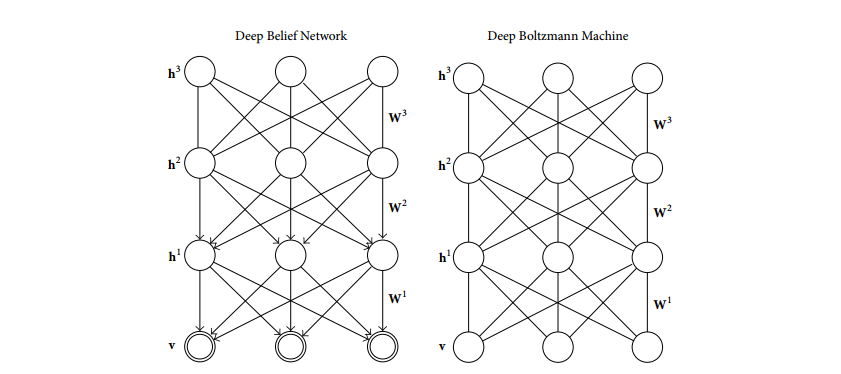
\includegraphics[scale=0.6]{fig2.png}
	\caption{深度信念网络(DBN)和深度玻尔兹曼机(DBM)。DBN的最顶部的两层是无向图构成,其余层是有向、自顶向下的连接层。在DBM中,所有连接都是无向的。}
	\label{fig:label}
\end{figure}
\subsubsection{限制玻尔兹曼机}
限制玻尔兹曼机([34,35])是一个无向图模型,它具有随机的可见变量$\bm{v}\in {0,1}^{D}$以及随机的影藏变量$\bm{h}\in \{0,1\}^F$,每个可见的变量都和不可见的变量相连接。RBM是玻尔兹曼机的一种变体,RBM限制了可见单元和不可见单元必须构成一个二分图,这个限制使得训练算法可以更加高效,尤其是基于梯度的对比散度算法[36]。

RBM定义了能量函数
$E:\{0,1\}^{D}\times \{0,1\}^{F} $
$\to$
$ \mathbb{R}$
\begin{equation}
	E(\bm{v},\bm{h};\theta) = -\sum_{i=1}^{D}\sum_{j=1}^{F}W_{ij}\nu_{i}h_{j}-\sum_{i=1}^{D}b_{i}\nu_{i}-\sum_{j=1}^{F}\alpha_{j}h_{j}
\end{equation}
其中$\theta = {\bm{\alpha},\bm{\beta},\bm{W}}$是模型参数;即$W_{ij}$表示可见单元$i$和隐藏单元$j$之间相互对称的影响项,$b_{i}$和$a_{j}$是偏置项。
可见和隐藏单元的联合分布为
\begin{equation}
	P(\bm{v},\bm{h};\theta) = \frac{1}{\mathcal{Z}(\theta)}exp(-E(\bm{v},\bm{h};\theta)),
	\mathcal{Z}(\theta)=\sum_{\bm{v}}\sum_{\bm{h}}exp(-E(\bm{v},\bm{h};\theta))
\end{equation}
其中$\mathcal{Z}(\theta)$是标准化的常量,隐藏单元$\bm{h}$和可见单元$\bm{h}$的条件分布由(5)(6)给出
\begin{equation}
	\begin{split}
		P(\bm{h}|\bm{v};\theta) = \prod_{j=1}^{F}p(h_{j}|\bm{v}),\\
		P(\bm{v}|\bm{h};\theta) = \prod_{i=1}^{D}p(v_{i}|\bm{h}).
	\end{split}
\end{equation}
考虑到一个观测的集合$\{\bm{V}_{n}\}^{N}_{n=1}$,对数似然对于模型参数的偏导数由(8)给出
\begin{equation}
	\frac{1}{N}\sum_{n=1}^{N}\frac{\partial logP(\bm{v_{n}};\theta)}{\partial W_{ij}}=\mathbb{E}_{P_{data}}[\nu_{i}h_{j}]-\mathbb{E}_{P_{model}}[\nu_{i}h_{j}],
\end{equation}
其中$\mathbb{E}_{P_{data}}$表示数据在分布为$P_{data}(\bm{h},\bm{v};\theta)=P(\bm{h}|\bm{v};\theta)P_{data}(\bm{v})$时的均值,$P_{data}(\bm{v})=(1/N)\sum_{n}\delta(\bm{v}-\bm{v}_{n})$是经验分布,$\mathbb{E}_{P_{model}}$是在模型定义分布下的均值,如式(6)所示。

RBMs的更多细节和实际训练方式的描述在[37]中给出,而且[38]讨论了训练RBMs的困难性及其内在原因,并提出了一种新的自适应学习速率和增强梯度的算法,以便解决前文中提到的问题。

\subsubsection{深度信念网络}
深度信念网络(DBNs)是一个概率生成式模型,它给出了观测到的数据和标签的联合概率分布。它们由堆叠的RBMs组成,通过贪心算法训练,文献[39]中有详细说明。DBN最初采用高效的逐层贪心学习策略来初始化深度网络,然后根据期望的输出同时调整所有权值。DBNs是能够学习到训练数据的深层层次表示的图模型。它会按如下方法建立观测向量$\bm{x}$和$l$个隐藏层$\bm{h}^{k}$的联合概率分布。
\begin{equation}
	P(\bm{x},\bm{h}^{1},\cdots,\bm{h}^{l})=
	\left(
	\prod_{k=0}^{l-2}P(\bm{h}^{k}|\bm{h}^{k+1})
	\right)
	P(\bm{h}^{l-1},\bm{h}^{l}),
\end{equation}
其中$\bm{x}=\bm{h}^{0}$,$P(\bm{h}^{k}|\bm{h}^{k+1})$是可见单元在第$k$层在隐藏单元是第$k+1$层的条件下的条件概率,而$P(\bm{h}^{l-1}|\bm{h}^l)$是可见单元和隐藏单元在RBM顶层的联合概率分布。

逐层采用非监督的贪心训练的策略可以应用于以RBMs作为每层基础单元的DBNs[33,39]。以下简单描述一下这个过程:\\
(1)用训练RBM的方法训练第一层,将输入$\bm{x}=\bm{h}^{0}$作为它的的可见层。\\
(2)通过第一层得到输入的表征,以备输入到第二层。这个过程有两个方法,表征可以是$P(\bm{h}^{1}|\bm{h}^{0})$的平均激活,或者是$P(\bm{h}^{1}|\bm{h}^{0})$中的采样。\\
(3)用训练RBM方法训练第二层,将转化后的数据(样本或者是平均激活)作为本层RBM可见层的训练样本。
(4)在每一层上重复步骤(2)(3),每次逐层向上传导样本或者平均激活。
(5)使用DBN的对数似然或通过有监督的训练法则调整深层结构中的所有参数(之后增加一层学习机制将学习到的表征转化为预测输出,例如线性分类器)\\
上述的贪心学习过程有两个主要的优点[40]。第一,它解决了选择初始权值的困难,从而使得网络能够合理地初始化,因为很多情况下初始值选择不当会导致模型收敛到局部最优。第二,非监督的学习方法无需对数据进行标注。然而,DBN也有很多不足,比如训练DBN的计算开销以及以及优化方法是不够清晰的最大似然估计法[41]。此外,DBN的一个很大的缺点是它不能将图片以二维输入,这会严重影响它在计算机视觉和多媒体分析领域中的表现。不过,一个DBN的变种,卷积深度信念网络(CDBN)([42,43]),通过引入卷积RBMs使用了像素点及其领域的空间信息,从而在高维的图片中可以得到平移不变的生成式模型[44]。
\subsubsection{深度玻尔兹曼机}
深度玻尔兹曼机(DBMs)[45]是另一种使用RBM作为基础单元的深度模型。DBMs的结构不同之处在于顶端的两层是无向图模型而下层是有向图模型,尽管DBM的所有连接都是无向的。DBMs具有多层隐藏单元,这些单元在奇数层中与偶数层中是条件独立的,反之亦然。因此推理DBM的机理往往是复杂的。另外,选择互动的隐藏单元和可见单元会使得模型更加复杂。在网络训练的过程中,DBM同时在所有层进行非监督式地训练,使用随机最大似然(SML)代替最大似然法,SML基于在似然上最大化下界的算法,这种方法容易收敛到不好的局部最小值[45],使得一些单元形同虚设。因此,人们提出了一种基于贪心的逐层训练策略[47],主要以预训练的DBM层组成,与DBN很相似,即通过多层RBMs使用前一层的输出独立地训练每一层,最后再同时进行参数调整。

关于DBMs的优点,它可以捕捉输入数据的多层复杂表征,数据无需标注,可以非监督学习,也可以进行监督学习。一个用来区分DBMs和其他深度模型的特点是DBMs自带推理过程而非通常的自底向上再自顶向下的传导过程,因此更加有效地提取了输入数据的不确定信息。此外,在DBMs中,通过可变下界在最大似然目标下的梯度估计,可以同时对所有层的参数进行优化,在模型学习来源多样的数据时有很大的优势[48]。

至于DBMs的缺点,最重要的缺点之一就是,正如上文所提及的,大量的计算开销会使得模型在大规模数据集上无法有效训练。人们为此提出了一些提高DBMs效率的方法,包括使用分离的模型并初始化所有隐藏层的权值来加速推理过程[47,49],或者其他在预训练过程或训练过程上的改进[52,53]。

\subsection{多层(降噪)自动编码机}
多层自动编码机使用自编码器作为它的构建单元,就如同深度信念网络使用限制玻尔兹曼机作为组成单元一样,因而在探讨多层(降噪)自动编码机之前,需要先讨论自编码器和它的降噪版本。

\subsubsection{自编码器}
人们训练自编码器将输入$\bm{x}$编码成$\bm{r}(\bm{x})$,再通过$\bm{r}(\bm{x})$重建输入[33]。因此自编码器的输出就是自编码器的输入,输出向量和输入向量的维数是一样的。在这个过程中,目标是最小化重建误差,输入输出对应的码就是学习到的特征。如果模型中有一层线性隐藏层并使用均方差作为损失函数来训练网络,$k$个隐藏单元会学习输入的前$k$个主成分[54]。如果隐藏层是非线性的,自编码器就不同于主成分分析,可以提取出各个方面的输入分布[55],模型的参数被优化来最小化平均重建误差。重建误差的衡量方式有很多种,其中包括传统的均方差:
\begin{equation}
	L =
	\parallel \bm{x}-\bm{f}(\bm{r}(\bm{x})) \parallel ^{2},
\end{equation}
其中函数$\bm{f}$是解码器,而$\bm{f}(\bm{r}(\bm{x}))$是重建过程。
如果输入是比特向量或者比特概率,则重建的损失函数可以由交叉熵表示:
\begin{equation}
	L = -\sum_{i}\bm{x}_{i}log \bm{f}_{i}(\bm{r}(\bm{x}))+(1-\bm{x}_{i}) log (1-\bm{f}_{i}(\bm{r}(\bm{x}))).
\end{equation}
目标是使得$\bm{r}(\bm{x})$的向量表示能够反映数据之间的主要差异,类似于主成分分析(PCA)。由于$\bm{r}(\bm{x})$必定会损失信息,所以我们不可能成功重建出所有的输入$\bm{x}$。之前提到的优化方法可以使得在重建与训练集同分布的测试集时误差较小,但是在任意从样本空间中抽取输入时会导致较大的误差。

\subsubsection{降噪自编码器}
降噪自编码器[56]是自编码器的随机版本,它将输入随机腐蚀,未腐蚀的输入仍然作为重建的输出目标。简单来说,在降噪自编码器的函数中有两个主要方面:第一步它将输入进行编码(也就是保留输入中的信息),第二步还原自编码器在输入上腐蚀过程造成的影响(见图3)。后者通过捕捉输入的统计学信息来完成。降噪编码器使用对数似然法,相比其它生成式模型能够得到更低的下界。
\begin{figure}[ht]
	\centering
	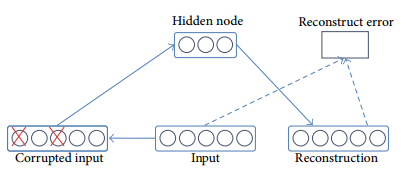
\includegraphics[scale=0.6]{fig3.png}
	\caption{降噪自编码器[56]}
	\label{fig:label}
\end{figure}
在[56]中,随机腐蚀过程随机将一些输入设为0,然后降噪自编码器对一些随机选择的输入,试图通过没有腐蚀的值来预测腐蚀的值。本质上来说,通过其余部分预测一个变量的任何子集是一个使模型学习到变量集合的联合分布的充分条件。值得一提的是使用自编码器来降噪早在[57]中被介绍,但是主要突破([56])还是在于成功演示了使用这种方法进行深度网络的非监督学习和将降噪自编码器与生成式模型二者结合。

\subsubsection{多层降噪自编码器}
多层降噪自编码器,通过将前一层的输出作为当前层降噪编码器的输入来构建深度网络。这个结构的非监督预训练是逐层进行的,每一层都作为一个降噪编码器来训练,目标是使得重建输入(也就是上一层的输出)的误差最小化。当前$k$层训练完成后,就可以训练第$(k+1)$层,因为第$(k+1)$层的输入输出已经由之前的层给出。

当预训练完成后,网络将进入第二阶段——调整阶段。这时将进行有监督的参数调整,目标是使得整个任务的预测误差最小化,为此,在第一阶段的输出层之上增加了一层逻辑回归层,之后这个网络就像一个多层的感知器一样训练,只需考虑每一个自编码器的编码过程。整个阶段是有监督的,因为目标类别在训练的过程中会使用到。

显然,训练多层自编码器和训练之前所述的深度信念网络是一样的,只是使用自编码器代替了限制玻尔兹曼机。一些比较试验表明深度信念网络要优于多层编码器([58,59]),但也不尽然,其中值得一提的是DBNs和多层降噪自编码器的对比[56]。

自编码器作为深度结构中基本的非监督组成部分的优点之一是,不同于RBMs,它在训练法则在参数上连续的前提下,允许任何参数化的网络层次。然而,SAs的一个缺点是它与生成式模型不相符合,在RBMs和DBNs这些生成式模型中,可以从训练过程中抽取样本来检查网络的输出。
\subsection{小节}
目前深度学习模型的一些缺点和局限已经在之前的小节中讨论过。比较这些模型(模型一览见表2),CNNs在当前的计算机视觉基准数据(如MNIST)上的表现优于DBNs。在一些无法可视化的数据集上,DBNs表现优于其他模型,但是难以准确估计联合分布概率以及训练DBN的巨大开销都是DBNs的缺点。CNNs的一个主要优势就是“特征学习”,能够绕过人工特征提取,这对于其他网络也是必要的。不过,CNNs的特征是自主学习的,所以它对标注的正确性依赖很高。然而DBNs/DBMs和SAs都对标注依赖不高并能进行非监督学习。另一方面,自编码机的一个缺点是如果第一层的误差过大的话会十分影响模型的整体性能。而降噪自编码器[56],从腐蚀的输入中得到正确的输入,这会使得网络习得输入的分布特点。就训练的效率而言,仅仅SAs是可以实时训练的,而CNNs和DBNs/DBMs的训练过程会消耗大量时间。最后,CNNs的一个优点是它在某些变换下的不变性,比如平移、伸缩和旋转。对这些变换的不变性是CNNs的重要特性,尤其是在计算机视觉领域(如目标检测),因为这允许直接从视觉输入提取目标的身份或种类,因而使得网络能够在实际像素大小不同的图片中有效地识别同一物体。
%\linespread{1.5}
\begin{table}
	\centering
	\caption{CNNs,DBNs/DBMs和SdAs在各个特性上的比较,加号表示具有该特性,减号表示在该项表现不好}
	\begin{tabular}{cccc}
		\toprule  %添加表格头部粗线
		模型特性             & CNNs & DBNs/DBMs & SdAs \\
		\midrule  %添加表格中横线
		非监督学习           & -    & +         & +    \\
		训练效率             & -    & -         & +    \\
		特征学习             & +    & -         & -    \\
		伸缩/旋转/平移不变性 & +    & -         & -    \\
		泛化性能             & +    & +         & +    \\
		\bottomrule %添加表格底部粗线
	\end{tabular}
\end{table}
\section{计算机视觉中的应用}
这一部分,本文总结了一些使用深度学习方法解决计算机视觉中关键任务的例子,比如目标检测,人脸识别,行为识别和人体姿态估计。
\subsection{目标检测}
目标检测是在图像和视频中检测语义上某类目标的实例(比如人,飞机或鸟)(如图4)。目标检测框架的一个通用的方法是创造大量的候选窗口来使用CNNs提取其中的特征,然后进行分类。例如,[32]中的方法采用了选择性搜索[60]得到对象备选窗口,对每个窗口用CNNs提取其特征,然后使用SVM基于这些特征判断目标是否在窗口内。大量基于区域CNN特征的概念在[32]中提出。采用区域CNN特征的研究往往有很好的准确性[61,62];然而,也有大量的研究致力于提高区域CNN方法的性能,其中的一些已经成功找到目标位置的大致估计但不能确定目标的精确位置[63],因此,这个方法通常用来进行联合目标检测,结合语义分割方法[64-66]通常能得到不错的结果。


\begin{figure}[ht]
	\centering
	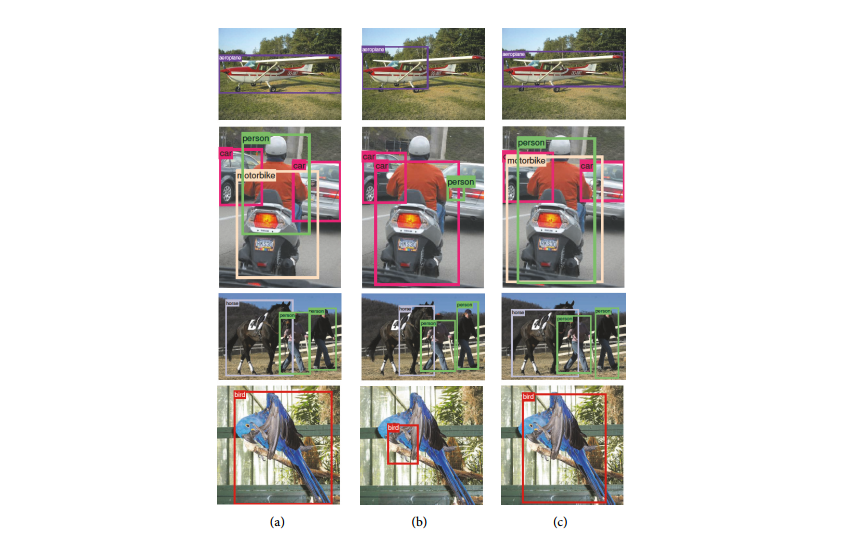
\includegraphics[scale=0.6]{fig4.png}
	\caption{目标检测的结果[66].(a)正确答案.(b)[32]的结果.(c)[66]的结果}
	\label{fig:label}
\end{figure}
主要的深度学习目标检测的方法使用的是CNNs的一个变种,例如[8,67,68](其中采用了def-pooling池化层并提出了新的学习策略),[9](弱监督级联CNNs)和[69](子类感知CNNs)。然而,也有一些目标检测研究尝试了其他的深度模型。例如[70]结合显著性机制和DBN提出了在远景图片中粗略定位目标的方法;[71]提出了一种3D目标识别的新DBN模型,其中顶层模型是一个3阶的玻尔兹曼机,结合生成梯度和判别梯度的混合算法进行训练。[72]使用了一种融合深度学习方法,而[73]研究了一种半监督深度模型的表征能力。最后[74]提出了多层自编码机来识别医学图像中的各种人体组织,[75]提出了显著性主导的多层自编码器来检测短片中的重要目标。
\subsection{人脸识别}
人脸识别是最热门的计算视觉任务之一,具有极大的商业前景。人们提出了各种各样的人工特征提取方法[76-79];这些特征提取器将人脸转化成一个低维的矩阵或向量表达,然后用分类器对其进行分类预测。CNNs的特征学习能力和变换不变性给人脸识别领域带来了重大变革。[80]首次使用CNNs进行人脸识别;如今light CNN[81]和VGG Face Descriptor[82]是十分先进的人脸识别网络;[44]中卷积DBN也在人脸确认方向取得了重要成果。

此外谷歌的FaceNet[83]和Facebook的Deep-Face[84]也都基于CNNs,DeepFace[84]建立了人脸的3D模型,标准化的数据被输入到一层卷积-池化-卷积的过滤器,然后经过3层局部连接层和2层全连接层得到预测的分类结果。尽管DeepFace表现很好,但是它的表征解释性不强,因为在运行过程中同一个人的面部不一定会聚一类。另一方面FaceNet在表征上定义了三元损失函数,使得训练过程可以将同一个人的人脸表征聚为一类。此外,CNNs也是OpenFace[85]的核心,Openface是一个开源的人脸识别工具,准确性略低于其他模型,但因为其轻量、迅速适合在手机上使用。

\subsection{行为识别}
行为识别是一个受到广泛关注的研究方向[86,87]。近年来,学者们发表了很多基于深度学习模型的人类行为识别成果[88]。在[89]中,深度学习被用来对一段视频进行复杂的事件检测和识别:首先,人们用显著图来检测和定位事件,之后使用深度学习预训练特征找到最重要的框架及其对应的事件。在[90]中作者成功地使用基于CNN的方法进行沙滩排球的行为检测,方法与[91]中从大规模视频数据中进行事件分类相似;[92]建立了一个CNN模型来对手机传感器数据进行行为检测。[12]的作者使用了半径-边缘边界作为深度CNN的正则项,有效提升了CNN在行为识别上的泛化性能。[13]中,作者细致研究了CNN作为精细活动的联合特征提取器和分类模型的应用效果,他们发现由于大的组内方差和小的组内方差以及每类活动训练样本有限等问题的存在,直接将NamgeNet训练出的特征交给SVM分类是一个好的选择。

受到模型的适应性以及各种不同传感器的可用性的驱动,在人类行为识别领域,融合多种特征越来越受到人们青睐。[93]中,作者融合了外貌和动作特征来识别人群中小组的行为,其数据来源于网络。为了结合不同的模型,很多作者应用了多任务学习模型。[94]使用各种特征的组合来对复杂的时间进行识别,将问题分为两个子问题:首先估计事件识别所需的最重要的一些特征,然后使用与/或图结构将不同的特征结合。也有很多研究将多个模型组合在一起,在[95]中,作者提出了多峰多流的深度学习框架来解决自我行为识别问题,在短片和传感器数据上使用双重CNNs和LSTM结构。融合CNN和LSTM结构的方法也出现在[96]中。最后[97]使用了DBNs进行行为检测,并以短片作为输入。
\subsection{人体姿态估计}
人体姿态估计的目标是确定图片、或一系列图片、深度影像或骨架数据(由运动检测硬件得到[98])中的人的位置。由于人轮廓和外貌的多样性,照明问题,背景杂乱的问题,人体姿态估计是一个非常具有挑战性的任务。在深度学习的浪潮开始之前,姿态估计基于对身体部分的检测,例如通过绘图结构[99]。

人体姿态估计的深度学习模型,可以根据输入图像的处理方式分为整体的和部分的方法。整体处理以全局的方法完成任务而不为每个部分定义明确的模型和空间关系。DeepPos[14]是一种整体模型,它将人体姿态估计方法规划为回归问题而不明确定义图模型或者局部探测器。然而基于整体的模型往往局限于高精度的区域,因为直接对图片中复杂的姿态向量进行回归是十分困难的。

另一方面,局部模型独立地探测人体的不同部分,再由一个图模型整合这些空间信息。在[15]中,为了学习到局部出现和空间关系的条件概率,作者使用局部的小块图像和背景块来训练CNN而非使用整张图片。[100]中的方法训练多个小的CNNs来分别对身体部分进行二分类,然后用一个高阶弱空间模型来剔除异常值保证姿态的全局一致性。最后,[101]设计了多分辨的CNN来对身体的每个部分计算热力图似然回归,随后使用一个隐性图模型提高联合一致性。

\subsection{数据集}
深度学习方法的应用能力在很多应用场景中的大规模数据集上都有评测。除去研究的情况,主要应用领域是在(自然)图像中。下面是对一些实用的数据集的整理:\\
(1)灰度图\\
使用最频繁的灰度图数据集是MNIST[20]和它的变种,即NIST和扰动NIST。它的应用场景是手写数字识别。\\
(2)RGB图\\
Caltech RGB图集[102],例如Caltech 101/Caltech 256和Caltech Silhouettes,包括不同的101/256类物体。CIFAR数据集[103]包括上千张$32\times 32$不同类的彩色图片,COIL数据集[104]包括不同物体旋转每一度之后的图片。\\
(3)高光谱图像\\
SCIEN高光谱数据集[105]和基于AVIRIS传感器的数据集[106]。\\
(4)面部特征图集\\
Adience标准数据集可以用来做面部的属性验证,这些属性包括年龄和性别。非限制场景下的人脸识别[108]是另一个常用的数据集。\\
(5)医学图像\\
Chest X射线数据集[109]有112120幅来源于30805个病人的正面X射线造影,这些图片有14种疾病标签(某些图会有多个标签)。Lymph Node Detection和Segmentation数据集[110]包括纵膈和腹部的CT图像。\\
(6)视频\\
WR数据集[111,112]可以被用来作为流水线上的基于视频的行为识别[113],包括7种连续的工业作业。YouTube-8M[114]包含了8百万YouTube视频的URL以及4800种视频标签。\\

\section{总结}
近年来的深度学习狂潮很大程度源于其在计算机视觉领域的卓越成果。本文综述的三类深度学习的主要方法,即CNNs,包括DBNs和DBMs的“玻尔兹曼家族”,以及SdAs,都已经在各类计算机视觉任务上有优秀表现,比如目标检测,人脸识别,行为识别,人体姿态估计,图像检索和语义分割。然而每种方法都有其优点和缺点。CNNs有独特的图像特征提取能力,即在给定数据集上自动提取特征。CNNs对一些变换也具有不变性,这是其在计算机视觉应用中的一大优点。但另一方面,相比于DBNs/DBMs和SdAs,CNNs严重依赖带有标签的数据,而前者可以在非监督下进行训练。这些模型中CNNs和DBNs/DBMs在训练时都需要大量的计算资源,而SdAs相对能训练过程更快。

作为结束语,尽管光明的前景使得对深度学习模型的研究越来越多,我们仍然需要面临很多挑战,尤其是在基础理论上能否清楚地解释优化方法、给定任务下模型结构的选择标准,深刻地理解给定任务中某个特定结构或算法是否有效。这些都是吸引未来机器学习研究社区的重要课题。

\section*{参考文献}

[1] W. S. McCulloch and W. Pitts, “A logical calculus of the ideas
immanentinnervousactivity,” Bulletin of Mathematical Biology,
vol. 5, no. 4, pp. 115–133, 1943.


[2] Y. LeCun, B. Boser, J. Denker et al., “Handwritten digit recognition with a back-propagation network,” in Advances in Neural
Information Processing Systems 2 (NIPS*89), D. Touretzky, Ed.,
Denver, CO, USA, 1990.


[3] S. Hochreiter and J. Schmidhuber, “Long short-term memory,”
Neural Computation, vol. 9, no. 8, pp. 1735–1780, 1997.


[4] G. E. Hinton, S. Osindero, and Y.-W. Teh, “A fast learning
algorithm for deep belief nets,” Neural Computation, vol. 18, no.
7, pp. 1527–1554, 2006.


[5] TensorFlow, Available online: https://www.tensorfow.org.


[6] B. Frederic, P. Lamblin, R. Pascanu et al., “Teano: new features
and speed improvements,” in Deep Learning and Unsupervised Feature Learning NIPS 2012 Workshop, 2012, http://deeplearning.net/sofware/theano/.


[7] Mxnet, Available online: http://mxnet.io.


[8] W. Ouyang, X. Zeng, X. Wang et al., “DeepID-Net: Object
Detection with Deformable Part Based Convolutional Neural
Networks,” IEEE Transactions on Pattern Analysis and Machine
Intelligence, vol. 39, no. 7, pp. 1320–1334, 2017.


[9] A. Diba, V. Sharma, A. Pazandeh, H. Pirsiavash, and L. V. Gool,
“Weakly Supervised Cascaded Convolutional Networks,” in
Proceedings of the 2017 IEEE Conference on Computer Vision and
Pattern Recognition (CVPR), pp. 5131–5139, Honolulu, HI, July
2017.


[10] N. Doulamis and A. Voulodimos, “FAST-MDL: Fast Adaptive
Supervised Training of multi-layered deep learning models for
consistent object tracking and classifcation,” in Proceedings of
the 2016 IEEE International Conference on Imaging Systems and
Techniques, IST 2016, pp. 318–323, October 2016.


[11] N. Doulamis, “Adaptable deep learning structures for object
labeling/tracking under dynamic visual environments,” Multimedia Tools and Applications, pp. 1–39, 2017.


[12] L. Lin, K. Wang, W. Zuo, M. Wang, J. Luo, and L. Zhang, “A deep
structured model with radius-margin bound for 3D human
activity recognition,” International Journal of Computer Vision,
vol. 118, no. 2, pp. 256–273, 2016.


[13] S. Cao and R. Nevatia, “Exploring deep learning based solutions
in fne grained activity recognition in the wild,” in Proceedings
of the 2016 23rd International Conference on Pattern Recognition
(ICPR), pp. 384–389, Cancun, December 2016.


[14] A. Toshev and C. Szegedy, “DeepPose: Human pose estimation
via deep neural networks,” in Proceedings of the 27th IEEE
Conference on Computer Vision and Pattern Recognition, CVPR
2014, pp. 1653–1660, USA, June 2014.


[15] X. Chen and A. L. Yuille, “Articulated pose estimation by a
graphical model with image dependent pairwise relations,” in
Proceedings of the NIPS, 2014.


[16] H. Noh, S.Hong, and B.Han, “Learning deconvolution network
for semantic segmentation,” in Proceedings of the 15th IEEE
International Conference on Computer Vision, ICCV 2015, pp.
1520–1528, Santiago, Chile, December 2015.


[17] J. Long, E. Shelhamer, and T. Darrell, “Fully convolutional networks for semantic segmentation,” in Proceedings of the IEEE
Conference on Computer Vision and Pattern Recognition (CVPR
’15), pp. 3431–3440, IEEE, Boston, Mass, USA, June 2015.


[18] D. H. Hubel and T. N. Wiesel, “Receptive felds, binocular
interaction, and functional architecture in the cat’s visual
cortex,” Te Journal of Physiology, vol. 160, pp. 106–154, 1962.


[19] K. Fukushima, “Neocognitron: a self-organizing neural network model for a mechanism of pattern recognition unafected
by shif in position,” Biological Cybernetics, vol. 36, no. 4, pp.
193–202, 1980.


[20] Y. LeCun, L. Bottou, Y. Bengio, and P. Hafner, “Gradient-based
learning applied to document recognition,” Proceedings of the
IEEE, vol. 86, no. 11, pp. 2278–2323, 1998.
Computational Intelligence and Neuroscience 11


	[21] Y. LeCun, B. Boser, J. S. Denker et al., “Backpropagation applied
to handwritten zip code recognition,” Neural Computation, vol.
1, no. 4, pp. 541–551, 1989.


[22] M. Tygert, J. Bruna, S. Chintala, Y. LeCun, S. Piantino, and A.
Szlam, “A mathematical motivation for complex-valued convolutional networks,” Neural Computation, vol. 28, no. 5, pp. 815–
825, 2016.


[23] M. Oquab, L. Bottou, I. Laptev, and J. Sivic, “Is object localization for free? - Weakly-supervised learning with convolutional
neural networks,” in Proceedings of the IEEE Conference on
Computer Vision and Pattern Recognition, CVPR 2015, pp. 685–
694, June 2015.


[24] C. Szegedy, W. Liu, Y. Jia et al., “Going deeper with convolutions,” in Proceedings of the IEEE Conference on Computer Vision
and Pattern Recognition (CVPR ’15), pp. 1–9, Boston, Mass, USA,
June 2015.


[25] Y. L. Boureau, J. Ponce, and Y. LeCun, “A theoretical analysis
of feature pooling in visual recognition,” in Proceedings of the
ICML, 2010.


[26] D. Scherer, A. Muller, and S. Behnke, “Evaluation of pooling ¨
operations in convolutional architectures for object recognition,” Lecture Notes in Computer Science (including subseries
Lecture Notes in Artifcial Intelligence and Lecture Notes in
Bioinformatics): Preface, vol. 6354, no. 3, pp. 92–101, 2010.


[27] H. Wu and X. Gu, “Max-Pooling Dropout for Regularization of
Convolutional Neural Networks,” in Neural Information Processing, vol. 9489 of Lecture Notes in Computer Science, pp. 46–
54, Springer International Publishing, Cham, 2015.


[28] K. He, X. Zhang, S. Ren, and J. Sun, “Spatial Pyramid Pooling in
Deep Convolutional Networks for Visual Recognition,” in Computer Vision – ECCV 2014, vol. 8691 of Lecture Notes in Computer
Science, pp. 346–361, Springer International Publishing, Cham,
2014.


[29] K. He, X. Zhang, S. Ren, and J. Sun, “Spatial pyramid pooling in
convolutional networks for visual recognition,” IEEE Transactions on Pattern Analysis and Machine Intelligence, vol. 37, no. 9,
pp. 1904–1916, 2015.


[30] W. Ouyang, X. Wang, X. Zeng et al., “DeepID-Net: Deformable
deep convolutional neural networks for object detection,” in
Proceedings of the IEEE Conference on Computer Vision and
Pattern Recognition, CVPR 2015, pp. 2403–2412, USA, June 2015.


[31] A. Krizhevsky, I. Sutskever, and G. E. Hinton, “Imagenet classifcation with deep convolutional neural networks,” in Proceedings
of the 26th Annual Conference on Neural Information Processing
Systems (NIPS ’12), pp. 1097–1105, Lake Tahoe, Nev, USA,
December 2012.


[32] R. Girshick, J. Donahue, T. Darrell, and J. Malik, “Rich feature hierarchies for accurate object detection and semantic
segmentation,” in Proceedings of the 27th IEEE Conference on
Computer Vision and Pattern Recognition (CVPR ’14), pp. 580–
587, Columbus, Ohio, USA, June 2014.


[33] Y. Bengio, “Learning deep architectures for AI,” Foundations
and Trends in Machine Learning, vol. 2, no. 1, pp. 1–27, 2009.


[34] P. Smolensky, “Information processing in dynamical systems:
Foundations of harmony theory,” in In Parallel Distributed
Processing: Explorations in the Microstructure of Cognition, vol.
1, pp. 194–281, MIT Press, Cambridge, MA, USA, 1986.


[35] G. E. Hinton and T. J. Sejnowski, “Learning and Relearning in
Boltzmann Machines,” vol. 1, p. 4.2, MIT Press, Cambridge, MA,
1986.


[36] M. A. Carreira-Perpinan and G. E. Hinton, “On contrastive
divergence learning,” in Proceedings of the tenth international
workshop on artifcial intelligence and statistics., NP: Society for
Artifcial Intelligence and Statistics, pp. 33–40, 2005.


[37] G. Hinton, “A practical guide to training restricted Boltzmann
machines,” Momentum, vol. 9, p. 926, 2010.


[38] K. Cho, T. Raiko, and A. Ilin, “Enhanced gradient for training
restricted Boltzmann machines,” Neural Computation, vol. 25,
no. 3, pp. 805–831, 2013.


[39] G. E. Hinton and R. R. Salakhutdinov, “Reducing the dimensionality of data with neural networks,” American Association
for the Advancement of Science: Science, vol. 313, no. 5786, pp.
504–507, 2006.


[40] I. Arel, D. C. Rose, and T. P. Karnowski, “Deep machine learning—a new frontier in artifcial intelligence research,” IEEE
Computational Intelligence Magazine, vol. 5, no. 4, pp. 13–18,
2010.


[41] Y. Bengio, A. Courville, and P. Vincent, “Representation learning: a review and new perspectives,” IEEE Transactions on
Pattern Analysis and Machine Intelligence, vol. 35, no. 8, pp.
1798–1828, 2013.


[42] H. Lee, R. Grosse, R. Ranganath, and A. Y. Ng, “Convolutional
deep belief networks for scalable unsupervised learning of
hierarchical representations,” in Proceedings of the 26th Annual
International Conference (ICML ’09), pp. 609–616, ACM, Montreal, Canada, June 2009.


[43] H. Lee, R. Grosse, R. Ranganath, and A. Y. Ng, “Unsupervised
learning of hierarchical representations with convolutional
deep belief networks,” Communications of the ACM, vol. 54, no.
10, pp. 95–103, 2011.


[44] G. B. Huang, H. Lee, and E. Learned-Miller, “Learning hierarchical representations for face verifcation with convolutional
deep belief networks,” in Proceedings of the IEEE Conference on
Computer Vision and Pattern Recognition (CVPR ’12), pp. 2518–
2525, June 2012.


[45] R. Salakhutdinov and G. Hinton, “Deep boltzmann machines,”
in Proceedings of the International Conference on Artifcial
Intelligence and Statistics, vol. 24, pp. 448–455, 2009.


[46] L. Younes, “On the convergence of Markovian stochastic algorithms with rapidly decreasing ergodicity rates,” Stochastics and
Stochastics Reports, vol. 65, no. 3-4, pp. 177–228, 1999.


[47] R. Salakhutdinov and H. Larochelle, “Efcient learning of deep
Boltzmann machines,” in Proceedings of the AISTATS, 2010.


[48] N. Srivastava and R. Salakhutdinov, “Multimodal learning
with deep Boltzmann machines,” Journal of Machine Learning
Research, vol. 15, pp. 2949–2980, 2014.


[49] R. Salakhutdinov and G. Hinton, “An efcient learning procedure for deep Boltzmann machines,” Neural Computation, vol.
24, no. 8, pp. 1967–2006, 2012.


[50] R. Salakhutdinov and G. Hinton, “A better way to pretrain Deep
Boltzmann Machines,” in Proceedings of the 26th Annual Conference on Neural Information Processing Systems 2012, NIPS 2012,
pp. 2447–2455, usa, December 2012.


[51] K. Cho, T. Raiko, A. Ilin, and J. Karhunen, “A two-stage pretraining algorithm for deep boltzmann machines,” Lecture Notes in
Computer Science (including subseries Lecture Notes in Artifcial
Intelligence and Lecture Notes in Bioinformatics): Preface, vol.
8131, pp. 106–113, 2013.


[52] G. Montavon and K. Muller, “Deep Boltzmann Machines and ¨
the Centering Trick,” in Neural Networks: Tricks of the Trade, vol.
7700 of Lecture Notes in Computer Science, pp. 621–637, Springer
Berlin Heidelberg, Berlin, Heidelberg, 2012.
12 Computational Intelligence and Neuroscience


	[53] I. Goodfellow, M. Mirza, A. Courville et al., “Multi-prediction
deep Boltzmann machines,” in Proceedings of the NIPS, 2013.


[54] H. Bourlard and Y. Kamp, “Auto-association by multilayer perceptrons and singular value decomposition,” Biological Cybernetics, vol. 59, no. 4-5, pp. 291–294, 1988.


[55] N. Japkowicz, S. J. Hanson, and M. A. Gluck, “Nonlinear autoassociation is not equivalent to PCA,” Neural Computation, vol.
12, no. 3, pp. 531–545, 2000.


[56] P. Vincent, H. Larochelle, Y. Bengio, and P.-A. Manzagol, “Extracting and composing robust features with denoising autoencoders,” in in Proceedings of the Twenty-ffh International
Conference on Machine Learning (ICML’08), W. W. Cohen, A.
McCallum, and S. T. Roweis, Eds., pp. 1096–1103, ACM, 2008.


[57] P. Gallinari, Y. LeCun, S. Tiria, and F. Fogelman-Soulie, “Memoires associatives distribuees,” in Proceedings of the in Proceedings of COGNITIVA 87, Paris, La Villette, 1987.


[58] H. Larochelle, D. Erhan, A. Courville, J. Bergstra, and Y. Bengio,
“An empirical evaluation of deep architectures on problems
with many factors of variation,” in Proceedings of the 24th
International Conference on Machine Learning (ICML ’07), pp.
473–480, Corvallis, Ore, UA, June 2007.


[59] Y. Bengio, P. Lamblin, D. Popovici, and H. Larochelle, “Greedy
layer-wise training of deep networks,” in Advances in Neural
Information Processing Systems (NIPS06), B. Sch, J. Platt, and.,
T. Hofman, and B. Scholkopf, Eds., vol. 19, pp. 153–160, MIT ¨
Press, 2007.


[60] J. R. R. Uijlings, K. E. A. Van De Sande, T. Gevers, and A. W. M.
Smeulders, “Selective search for object recognition,” International Journal of Computer Vision, vol. 104, no. 2, pp. 154–171,
2013.


[61] R. Girshick, “Fast R-CNN,” in Proceedings of the 15th IEEE
International Conference on Computer Vision (ICCV ’15), pp.
1440–1448, December 2015.


[62] S. Ren, K. He, R. Girshick, and J. Sun, “Faster R-CNN: Towards
Real-Time Object Detection with Region Proposal Networks,”
IEEE Transactions on Pattern Analysis and Machine Intelligence,
vol. 39, no. 6, pp. 1137–1149, 2017.


[63] J. Hosang, R. Benenson, and B. Schiele, “How good are detection proposals, really?” in Proceedings of the 25th British
Machine Vision Conference, BMVC 2014, gbr, September 2014.


[64] B. Hariharan, P. Arbelaez, R. Girshick, and J. Malik, “Simultane- ´
ous detection and segmentation,” in Computer Vision—ECCV
2014, vol. 8695 of Lecture Notes in Computer Science, pp. 297–
312, Springer, 2014.


[65] J. Dong, Q. Chen, S. Yan, and A. Yuille, “Towards unifed
object detection and semantic segmentation,” Lecture Notes in
Computer Science (including subseries Lecture Notes in Artifcial
Intelligence and Lecture Notes in Bioinformatics): Preface, vol.
8693, no. 5, pp. 299–314, 2014.


[66] Y. Zhu, R.Urtasun, R.Salakhutdinov, and S. Fidler, “SegDeepM:
Exploiting segmentation and context in deep neural networks
for object detection,” in Proceedings of the IEEE Conference on
Computer Vision and Pattern Recognition, CVPR 2015,pp.4703–
4711, USA, June 2015.


[67] J. Liu, N. Lay, Z. Wei et al., “Colitis detection on abdominal CT
scans by rich feature hierarchies,” in Proceedings of the Medical
Imaging 2016: Computer-Aided Diagnosis, vol. 9785 of Proceedings of SPIE, San Diego, Calif, USA, February 2016.


[68] G. Luo, R. An, K. Wang, S. Dong, and H. Zhang, “A Deep Learning Network for Right Ventricle Segmentation in Short:Axis
MRI,” in Proceedings of the 2016 Computing in Cardiology
Conference.


[69] T. Chen, S. Lu, and J. Fan, “S-CNN: Subcategory-aware convolutional networks for object detection,” IEEE Transactions on
Pattern Analysis and Machine Intelligence, 2017.


[70] W. Diao, X. Sun, X. Zheng, F. Dou, H. Wang, and K. Fu,
“Efcient Saliency-Based Object Detection in Remote Sensing
Images Using Deep Belief Networks,” IEEE Geoscience and
Remote Sensing Letters, vol. 13, no. 2, pp. 137–141, 2016.


[71] V. Nair and G. E. Hinton, “3D object recognition with deep
belief nets,” in Proceedings of the NIPS, 2009.


[72] N. Doulamis and A. Doulamis, “Fast and adaptive deep fusion
learning for detecting visual objects,” Lecture Notes in Computer
Science (including subseries Lecture Notes in Artifcial Intelligence
and Lecture Notes in Bioinformatics): Preface,vol.7585,no.3,pp.
345–354, 2012.


[73] N. Doulamis and A. Doulamis, “Semi-supervised deep learning
for object tracking and classifcation,” pp. 848–852.


[74] H.-C. Shin, M. R. Orton, D. J. Collins, S. J. Doran, and M. O.
Leach, “Stacked autoencoders for unsupervised feature learning
and multiple organ detection in a pilot study using 4D patient
data,” IEEE Transactions on Pattern Analysis and Machine
Intelligence, vol. 35, no. 8, pp. 1930–1943, 2013.


[75] J. Li, C. Xia, and X. Chen, “A benchmark dataset and saliencyguided stacked autoencoders for video-based salient object
detection,” IEEE Transactions on Image Processing, 2017.


[76] D.Chen,X.Cao,F.Wen,andJ.Sun,“Blessingofdimensionality:
high-dimensional feature and its efcient compression for face
verifcation,” in Proceedings of the 26th IEEE Conference on
Computer Vision and Pattern Recognition (CVPR ’13), pp. 3025–
3032, June 2013.


[77] X. Cao, D. Wipf, F. Wen, G. Duan, and J. Sun, “A practical transfer learning algorithm for face verifcation,” in Proceedings of the
14th IEEE International Conference on Computer Vision (ICCV
’13), pp. 3208–3215, December 2013.


[78] T. Berg and P. N. Belhumeur, “Tom-vs-Pete classifers and identity-preserving alignment for face verifcation,” in Proceedings
of the 23rd British Machine Vision Conference (BMVC ’12), pp.
1–11, September 2012.


[79] D. Chen, X. Cao, L. Wang, F. Wen, and J. Sun, “Bayesian face
revisited:ajointformulation,”in Computer Vision—ECCV 2012:
12th European Conference on Computer Vision, Florence, Italy,
October 7–13, 2012, Proceedings, Part III, vol. 7574 of Lecture
Notes in Computer Science, pp. 566–579, Springer, Berlin,
Germany, 2012.


[80] S. Lawrence, C. L. Giles, A. C. Tsoi, and A. D. Back, “Face
recognition: a convolutional neural-network approach,” IEEE
Transactions on Neural Networks and Learning Systems, vol. 8,
no. 1, pp. 98–113, 1997.


[81] X. Wu, R. He, Z. Sun, and T. Tan, A light CNN for deep face representation with noisy labels, https://arxiv.org/abs/1511.02683.


[82] O. M. Parkhi, A. Vedaldi, and A. Zisserman, “Deep Face Recognition,” in Proceedings of the British Machine Vision Conference
2015, pp. 41.1-41.12, Swansea.


[83] F. Schrof, D. Kalenichenko, and J. Philbin, “FaceNet: a unifed
embedding for face recognition and clustering,” in Proceedings
of the IEEE Conference on Computer Vision and Pattern Recognition (CVPR ’15), pp. 815–823, IEEE, Boston, Mass, USA, June
2015.


[84] Y. Taigman, M. Yang, M. Ranzato, and L. Wolf, “DeepFace: closing the gap to human-level performance in face verifcation,”
in Proceedings of the IEEE Conference on Computer Vision and
Pattern Recognition (CVPR ’14),pp.1701–1708,Columbus,Ohio,
USA, June 2014.
Computational Intelligence and Neuroscience 13


	[85] B. Amos, B. Ludwiczuk, and M. Satyanarayanan, “Openface: a
general-purpose face recognition library with mobile applications,” CMU-CS-16-118, CMU School of Computer Science,
2016.


[86] A. S. Voulodimos, D. I. Kosmopoulos, N. D. Doulamis, and T. A.
Varvarigou, “A top-down event-driven approach for concurrent
activity recognition,” Multimedia Tools and Applications, vol. 69,
no. 2, pp. 293–311, 2014.


[87] A. S. Voulodimos, N. D. Doulamis, D. I. Kosmopoulos, and T. A.
Varvarigou, “Improving multi-camera activity recognition by
employing neural network based readjustment,” Applied Artifcial Intelligence, vol. 26, no. 1-2, pp. 97–118, 2012.


[88] K. Makantasis, A. Doulamis, N. Doulamis, and K. Psychas,
“Deep learning based human behavior recognition in industrial workfows,” in Proceedings of the 23rd IEEE International
Conference on Image Processing, ICIP 2016, pp. 1609–1613,
September 2016.


[89] C. Gan, N. Wang, Y. Yang, D.-Y. Yeung, and A. G. Hauptmann,
“DevNet: A Deep Event Network for multimedia event detection and evidence recounting,” in Proceedings of the IEEE
Conference on Computer Vision and Pattern Recognition, CVPR
2015, pp. 2568–2577, USA, June 2015.


[90] T. Kautz, B. H. Groh, J. Hannink, U. Jensen, H. Strubberg, and
B. M. Eskofer, “Activity recognition in beach volleyball using a
DEEp Convolutional Neural NETwork: leveraging the potential
of DEEp Learning in sports,” Data Mining and Knowledge
Discovery, vol. 31, no. 6, pp. 1678–1705, 2017.


[91] A. Karpathy, G. Toderici, S. Shetty, T. Leung, R. Sukthankar,
and F.-F. Li, “Large-scale video classifcation with convolutional
neural networks,” in Proceedings of the 27th IEEE Conference on
Computer Vision and Pattern Recognition, (CVPR ’14), pp. 1725–
1732, Columbus, OH, USA, June 2014.


[92] C. A. Ronao and S.-B. Cho, “Human activity recognition with
smartphone sensors using deep learning neural networks,”
Expert Systems with Applications, vol. 59, pp. 235–244, 2016.


[93] J. Shao, C. C. Loy, K. Kang, and X. Wang, “Crowded Scene
Understanding by Deeply Learned Volumetric Slices,” IEEE
Transactions on Circuits and Systems for Video Technology, vol.
27, no. 3, pp. 613–623, 2017.


[94] K. Tang, B. Yao, L. Fei-Fei, and D. Koller, “Combining the right
features for complex event recognition,” in Proceedings of the
2013 14th IEEE International Conference on Computer Vision,
ICCV 2013, pp. 2696–2703, Australia, December 2013.


[95] S. Song, V. Chandrasekhar, B. Mandal et al., “Multimodal MultiStream Deep Learning for Egocentric Activity Recognition,” in
Proceedings of the 29th IEEE Conference on Computer Vision
and Pattern Recognition Workshops, CVPRW 2016, pp. 378–385,
USA, July 2016.


[96] R. Kavi, V. Kulathumani, F. Rohit, and V. Kecojevic, “Multiview
fusion for activity recognition using deep neural networks,”
Journal of Electronic Imaging, vol. 25, no. 4, Article ID 043010,
2016.


[97] H. Yalcin, “Human activity recognition using deep belief networks,” in Proceedings of the 24th Signal Processing and Communication Application Conference, SIU 2016, pp. 1649–1652, tur,
May 2016.


[98] A. Kitsikidis, K. Dimitropoulos, S. Douka, and N. Grammalidis,
“Dance analysis using multiple kinect sensors,” in Proceedings of
the 9th International Conference on Computer Vision Teory and
Applications, VISAPP 2014, pp. 789–795, prt, January 2014.


[99] P. F. Felzenszwalb and D. P. Huttenlocher, “Pictorial structures for object recognition,” International Journal of Computer
Vision, vol. 61, no. 1, pp. 55–79, 2005.


[100] A. Jain, J. Tompson, and M. Andriluka, “Learning human pose
estimation features with convolutional networks,” in Proceedings of the ICLR, 2014.


[101] J. J. Tompson, A. Jain, Y. LeCun et al., “Joint training of a convolutional network and a graphical model for human pose
estimation,” in Proceedings of the NIPS, 2014.


[102] L. Fei-Fei, R. Fergus, and P. Perona, “One-shot learning of object
categories,” IEEE Transactions on Pattern Analysis and Machine
Intelligence, vol. 28, no. 4, pp. 594–611, 2006.


[103] A. Krizhevsky and G. Hinton, Learning multiple layers of features from tiny images, 2009.


[104] S. A. Nene, S. K. Nayar, and H. Murase, Columbia object image
library (coil-20), 1996.


[105] T. Skauli and J. Farrell, “A collection of hyperspectral images for
imaging systems research,” in Proceedings of the Digital Photography IX, USA, February 2013.


[106] M. F. Baumgardner, L. L. Biehl, and D. A. Landgrebe, “220 band
aviris hyperspectral image data set: June 12, 1992 indian pine test
site 3,” Datasets, 2015.


[107] E. Eidinger, R. Enbar, and T. Hassner, “Age and gender estimation of unfltered faces,” IEEE Transactions on Information Forensics and Security, vol. 9, no. 12, pp. 2170–2179, 2014.


[108] G. B. Huang, M. Ramesh, T. Berg, and E. Learned-Miller,
“Labeled faces in the wild: A database for studying face recognition in unconstrained environments,” Tech. Rep., University
of Massachusetts, Amherst, 2007.


[109] X. Wang, Y. Peng, L. Lu, Z. Lu, M. Bagheri, and R. M. Summers,
“ChestX-Ray8: Hospital-scale chest x-ray database and benchmarks on weakly-supervised classifcation and localization of
common thorax diseases,” in Proceedings of the 2017 IEEE Conference on Computer Vision and Pattern Recognition (CVPR), pp.
3462–3471, Honolulu, HI, May 2017.


[110] A. Sef, L. Lu, A. Barbu, H. Roth, H.-C. Shin, and R. M. Summers, “Leveraging mid-level semantic boundary cues for automated lymph node detection,” Lecture Notes in Computer
Science (including subseries Lecture Notes in Artifcial Intelligence
and Lecture Notes in Bioinformatics): Preface, vol. 9350, pp. 53–
61, 2015.


[111] A. Voulodimos, D. Kosmopoulos, G. Vasileiou et al., “A dataset
for workfow recognition in industrial scenes,” in Proceedings of
the 2011 18th IEEE International Conference on Image Processing,
ICIP 2011, pp. 3249–3252, Belgium, September 2011.


[112] A. Voulodimos, D. Kosmopoulos, G. Vasileiou et al., “A threefold dataset for activity and workfow recognition in complex
industrial environments,” IEEE MultiMedia, vol. 19, no. 3, pp.
42–52, 2012.


[113] D. I. Kosmopoulos, A. S. Voulodimos, and A. D. Doulamis, “A
system for multicamera task recognition and summarization
for structured environments,” IEEE Transactions on Industrial
Informatics, vol. 9, no. 1, pp. 161–171, 2013.


[114] S. Abu-El-Haija et al., “YouTube-8M: A large-scale video classifcation benchmark,” Tech. Rep., 2016, https://arxiv.org/abs/
1609.08675.
\end{CJK}
\end{document}
\documentclass{article}
\usepackage{CJK}
\begin{document}
\begin{CJK}{UTF8}{gbsn}
	中文测试
\end{CJK}
\end{document}

